\documentclass[12pt, a4paper]{article} %mostra o tipo do documento
\usepackage[brazil]{babel} %permite escrever em português
\usepackage[utf8]{inputenc}
\usepackage[a4paper, textheight=9in, textwidth=6.3in]{geometry} %ajusta as margens
\usepackage[T1]{fontenc} %define a fonte das letras
\usepackage{color} %colore as letras
\usepackage{url} %inclui urls
\usepackage[pdfencoding=unicode]{hyperref} %transforma links em texto comum para clicar
\usepackage{amsmath, amssymb, amsthm, amsfonts} %permite fazer textos matemáticos
\usepackage{float} % permite mover tabelas e figuras para qualquer ponto da página
\usepackage{graphicx} %permite colocar imagens no documento
\usepackage{indentfirst} %Indenta o primeiro parágrafo do capítulo
\usepackage{multirow}
\setlength\parindent{24pt}
\def\changemargin#1#2{\list{}{\rightmargin#2\leftmargin#1}\item[]}
\let\endchangemargin=\endlist 

\title{Relatório EP5 - MAC0121}
\date{}
\author{João Gabriel Basi - $\text{N}^\circ$ USP: 9793801}
\begin{document}
\maketitle
\section{O programa}
O programa implementa uma IA capaz de jogar o jogo Hex, um jogo de tabuleiro onde os jogadores se alternam colocando uma peça de sua cor no tabuleiro, com o objetivo de fazer um caminho entre as bordas opostas do tabuleiro de sua cor. O primeiro a conseguir fazer um caminho vence.

\section{As funções}
	\subsection{No arquivo da main (hex.c)}
	\begin{itemize}
		\item \textit{show\_usage}: Mostra uma mensagem de erro na saída de erro de acordo com o número fornecido;
		\item \textit{play}: Faz uma jogada;
		\item \textit{beginGameLoop}: Começa o loop do jogo;
	\end{itemize}
	\subsection{BoardFuncs.h}
	Biblioteca de funções que implementam o tabuleiro e ajudam a manuseá-lo.
	\begin{itemize}
		\item \textit{BTile}: Struct que implementa uma casa do tebueiro;
		\item \textit{BoardCreate}: Cria um tabuleiro;
		\item \textit{freeBoard}: Desaloca um tabuleiro;
		\item \textit{printGame}: Imprime o tabuleiro na saída de erro;
		\item \textit{isValid}: Verifica se a posição do tabuleiro é válida;
		\item \textit{getWinner}: Verifica se alguém venceu;
		\item \textit{updateWeigths}: Atualiza os pesos das peças do tabuleiro.
	\end{itemize}
	\subsection{PathFinding.h}
	Biblioteca de funções que ajudam o programa na criação e no manuseio de
caminhos pelo tabuleiro.
	\begin{itemize}
		\item \textit{macro e macroAux}: Vetores que auxiliam o programa à achar caminhos pelo tabuleiro;
		\item \textit{PNode}: Struct que implementa um nó de lista ligada Path;
		\item \textit{Path}: Struct que implemneta uma cabeça de lista ligada para um caminho de posições do tabuleiro;
		\item \textit{PathDestroy}: Destroi uma lista ligada do tipo Path;
		\item \textit{Intersec}: Acha a primeira posição comum entre dois caminhos;
		\item \textit{findPath}: Acha um caminho entre as duas laterais opostas de uma cor;
		\item \textit{pathcmp}: Vê se dois caminhos são iguais.
	\end{itemize}
	\subsection{auxfuncs.h}
	Biblioteca de funções que ajudam o programa a manusear a memória e
resumir operações.
	\begin{itemize}
		\item \textit{N}: Define o tamanho do tabuleiro;
		\item \textit{INF}: Define infinito como sendo $2^{30}$;
		\item \textit{Pos}: Struct que armazena uma posição do tabuleiro;
		\item \textit{emalloc}: Aloca uma posição de memória e imprime uma mensagem de erro se der errado;
		\item \textit{criaMatriz}: Aloca uma matriz;
		\item \textit{freeMatriz}: Desaloca uma matriz;
		\item \textit{criaVetor}: Aloca um vetor;
		\item \textit{coltoi}: Transforma uma cor em um inteiro;
		\item \textit{troca}: Troca o conteúdo de duas variáveis.
	\end{itemize}

\section{Implementação da IA}
	\par Esse programa não foi baseado em nenhum outro algoritmo existente (ao menos eu não achei nenhum parecido). A ideia dele é achar o suposto caminho que o outro jogador está tentando construir e tentar barrá-lo, para isso só foi preciso implementar uma função que acha um caminho vantajoso (nem sempre é o melhor possível) para cada jogador e outra que acha uma posição em comum entre eles (no caso, como nunca há empates, pois um jogador precisa bloquear a passagem do outro para vencer, podemos garantir que sempre há uma posição em comum entre os dois caminhos).
	\subsection{Pesos}
		\par Primeiro damos dois pesos para cada célula do tabuleiro, um em relação às peças brancas e outro em relação às peças pretas. Se uma célula está vazia e tem vizinhos vazios, seu peso é 4 para as duas cores. Para cada peça branca colocada em sua vizinhança, seu peso para as brancas diminui em 2 e seu peso para as pretas aumenta em 2, e o peso para as pretas funciona analogamente. Cada casa vazia pode ter no máximo peso 8 e no mínimo peso 0. Para as casas ocupadas, o peso é definido como sendo 0, para a cor da peça que está lá, e INF para a cor oposta. Quanto menor o peso de uma casa em relção à uma cor, melhor ela é para essa cor.
	\subsection{Achando o caminho}
		\par Para achar um caminho, a função findPath chama a função partialFindPath em todas as posições de uma das bordas de um jogador, e a partialFindPath executa um backtracking recursivo a partir daquela posição. O backtracking tem uma prioridade de verificação para cada cor de peça e lado do tabuleiro, essa prioridade é calculada a parir dos vetores macro e macroAux, como mostram as figuras:
		\begin{center}
		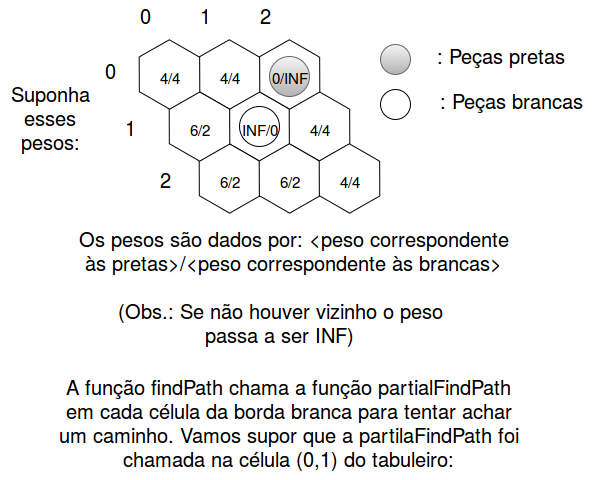
\includegraphics[scale=0.65]{pricalc1.png}\\
		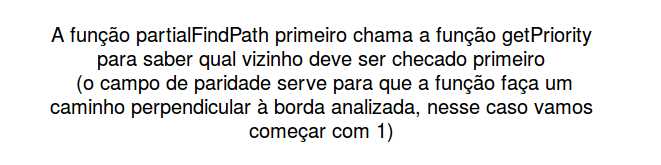
\includegraphics[scale=0.60]{pricalc25.png}\\
		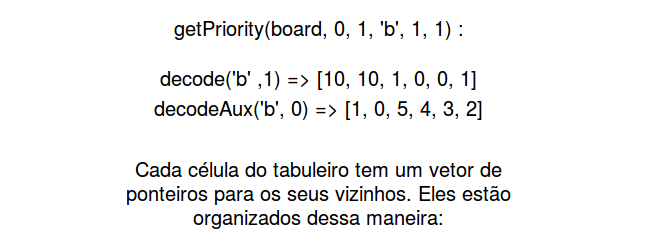
\includegraphics[scale=0.60]{pricalc2.png}\\
		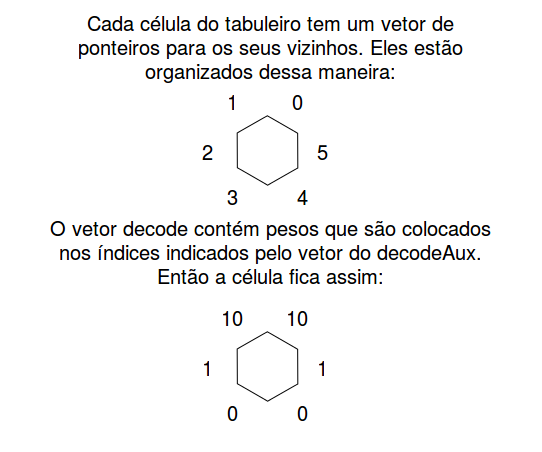
\includegraphics[scale=0.60]{pricalc3.png}\\
		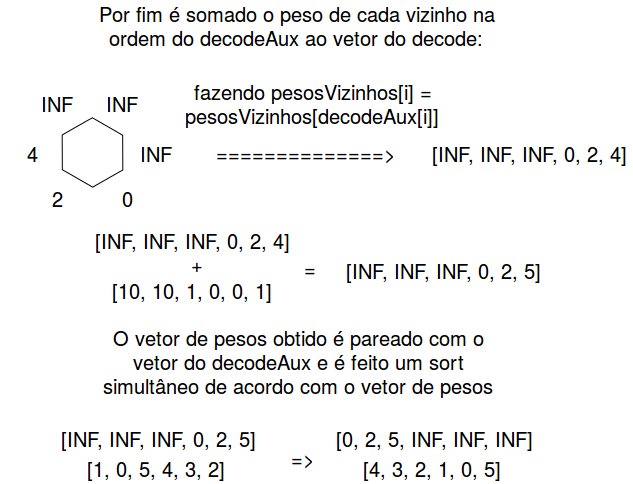
\includegraphics[scale=0.65]{pricalc4.png}\\
		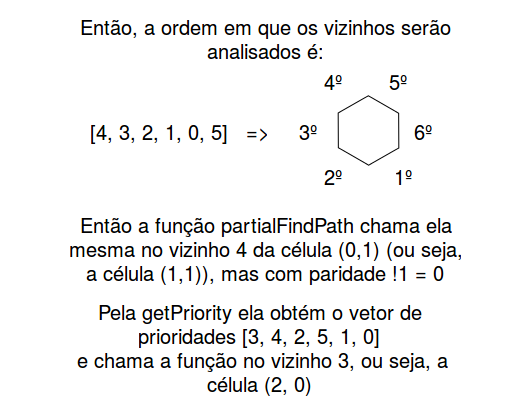
\includegraphics[scale=0.65]{pricalc5.png}\\
		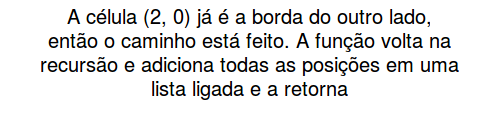
\includegraphics[scale=0.65]{pricalc6.png}\\
		\end{center}
		\par A interseção dos dois caminhos será onde o programa irá fazer sua jogada.

\section{Decisões de implementação}
	\par A minha intenção em criar o vetor macroAux é de alternar a prioridade de vizinhos simétricos e com o mesmo peso, achando caminhos tanto por um lado quanto por outro. Utilizei da estabilidade do bubble sort (realizado no getPriority) para obter prioridades diferentes para a mesma célula utilizando o vetor macroAux.
	\par O algoritmo, foi construído com partes de outros algoritmos. Por exemplo, o algoritmo que acha o caminho foi baseado no algoritmo A* (não implementei com fila pois não sabia como armazenar o caminho) e os pesos baseados em uma implementação do jogo pensando nas peças como resistores \cite{hexy}.

\section{Prós e contras}
	\subsection{Prós}
	\begin{itemize}
		\item Joga bem no começo, bloqueando os possíveis caminhos que o outro jogador possa fazer;
		\item Não achei nenhum algoritmo símples (como fazer um caminho em linha reta ou jogar aleatóriamente) que possa vencê-lo.
	\end{itemize}
	\subsection{Contras}
	\begin{itemize}
		\item Conforme as rodadas passam, ele fica mais confuso, pois não consegue achar direito os caminhos em meio à tantas peças, então as vezes faz jogadas que não adiantam em nada;
	\end{itemize}
\begin{thebibliography}{1}
\bibitem{hexy} Hexy \url{http://home.earthlink.net/~vanshel/VAnshelevich-01.pdf}
\end{thebibliography}
\end{document}